\documentclass[12pt,a4paper]{article}

\usepackage[utf8]{inputenc}
\usepackage[T1]{fontenc}
\usepackage[brazil]{babel}
\usepackage{geometry}
\usepackage{graphicx}
\usepackage{amsmath}
\usepackage{xcolor}
\usepackage{listings}
\usepackage{float}
\usepackage{fancyhdr}
\usepackage{hyperref}
\usepackage{ragged2e}
\usepackage{indentfirst}
\usepackage{enumitem}

\geometry{left=30mm,top=30mm,right=20mm,bottom=20mm}
\setlength{\parindent}{20pt}
\justifying
\pagestyle{fancy}
\fancyhf{}
\renewcommand{\headrulewidth}{0pt}
\fancyfoot[R]{\thepage}
\hypersetup{colorlinks=true,linkcolor=blue,urlcolor=blue}

\definecolor{codebackground}{HTML}{F7F7F7}
\definecolor{codecomment}{HTML}{008000}
\definecolor{codekeyword}{HTML}{0000AA}
\lstdefinestyle{cppstyle}{
  backgroundcolor=\color{codebackground},
  basicstyle=\ttfamily\footnotesize,
  commentstyle=\color{codecomment},
  keywordstyle=\color{codekeyword},
  breaklines=true,
  frame=single,
  numbers=left,
  numbersep=5pt,
  showstringspaces=false,
  tabsize=4
}
\lstset{style=cppstyle}

\begin{document}
\pagenumbering{gobble}

\begin{titlepage}
\begin{center}
  \IfFileExists{figs/logo-ufs1.jpg}{
\includegraphics[scale=0.10]{figs/logo-ufs1.jpg}\par\vspace{0.5cm}}{}
  \textbf{\large Universidade Federal de Sergipe}\\
  \textbf{\large Departamento de Computação}\\
  \textbf{\large Docente: Rafael Oliveira Vasconcelos}\\

  \vspace{1.5cm}
  \textbf{\Large Projeto Unidade 1}\\
  \vspace{0.5cm}
  \textbf{\large Sistemas Distribuídos -- T01 2026.2}\\

  \vfill
  \textbf{\large Discentes}\\
  Arthur Vinícius Costa Barreto\\
  Bruno Carvalho Santana Rocha\\
  Danilo Campos Deichmann\\
  Filipe Ciríaco Marcelino do Nascimento\\
  Sidnei Silva Gonçalves Junior\\

  \vfill
  São Cristóvão -- SE\\
  21 de outubro de 2026
\end{center}
\end{titlepage}
\newpage
\pagenumbering{arabic}

\section{Introdução}
O presente documento descreve a proposta técnica para o desenvolvimento de um Simulador de Bolsa de Valores Multiplayer, desenvolvido como requisito de avaliação da disciplina de Sistemas Distribuídos. O sistema permitirá a conexão simultânea de múltiplos investidores em um ambiente de mercado financeiro virtual, abordando desafios de consistência, concorrência e tolerância a falhas.

\section{Regras do Mercado, Ativos e Investidores}

\subsection{Perfil dos Investidores e Capital Inicial}
Cada jogador iniciará com um capital virtual de R\$ 10.000,00 e uma carteira vazia de ativos. Para focar a complexidade nos desafios de sistemas distribuídos (como concorrência e sincronização), o mercado operará com corretagem zero (sem taxas por transação) e sem limites de quantidade por negociação, desde que haja saldo ou ativos suficientes.

\subsection{Ativos Virtuais}
O mercado disponibilizará 4 ativos reais baseados na B3, representando diferentes setores da economia:
\begin{itemize}
    \item \textbf{PETR4:} Petrobras - Preço base: R\$ 35,00
    \item \textbf{VALE3:} Vale - Preço base: R\$ 68,00
    \item \textbf{ITUB4:} Itaú Unibanco - Preço base: R\$ 30,50
    \item \textbf{MGLU3:} Magazine Luiza - Preço base: R\$ 2,10
\end{itemize}

\subsection{Mecânica de Negociação e Eventos Econômicos}
As ordens seguirão o princípio de prioridade de preço e prioridade temporal no \textit{Matching Engine}. O mercado funcionará 24 horas por dia (sem interrupções na simulação). Para estimular a volatilidade, o sistema gerará ''Eventos Econômicos'' aleatórios a cada 10 minutos (ex: ''Boom Tecnológico'' ou ''umento de Juros'', impactando os preços de referência dos ativos e incentivando os investidores conectados a adaptarem as suas estratégias.


\section{Cronograma de Desenvolvimento}
O cronograma abaixo reflete as atividades distribuídas até as entregas:
\begin{itemize}
    \item \textbf{21/10/2026:} Entrega da Proposta, diagrama arquitetural, infraestrutura em contêineres e Protótipo funcional (login JWT, painel e envio em tempo real via STOMP).
    \item \textbf{Novembro/2026 (Semanas 1-2):} Integração completa do Matching Engine na memória com a base de dados relacional.
    \item \textbf{Novembro/2026 (Semanas 3-4):} Execução de testes de carga em larga escala, indução de falhas e refatoração arquitetural.
    \item \textbf{30/11/2026:} Apresentação final e entrega do código com documentação.
\end{itemize}

\section{Arquitetura Distribuída e Tecnologias}

\subsection{Arquitetura Proposta e Diagrama}
O sistema adota uma arquitetura modular em contêineres orquestrada via Docker Compose. O fluxo de comunicação baseia-se na interação do \textbf{Navegador (Home Broker)} servido por um contêiner \textbf{Nginx}, que roteia as requisições e a comunicação em tempo real para o \textbf{Backend Spring Boot (REST + STOMP)}. O Backend centraliza toda a lógica de negócio, a gestão de estado em memória para processamento rápido e persiste os dados consolidados num banco \textbf{PostgreSQL}.

\begin{figure}[H]
    \centering
    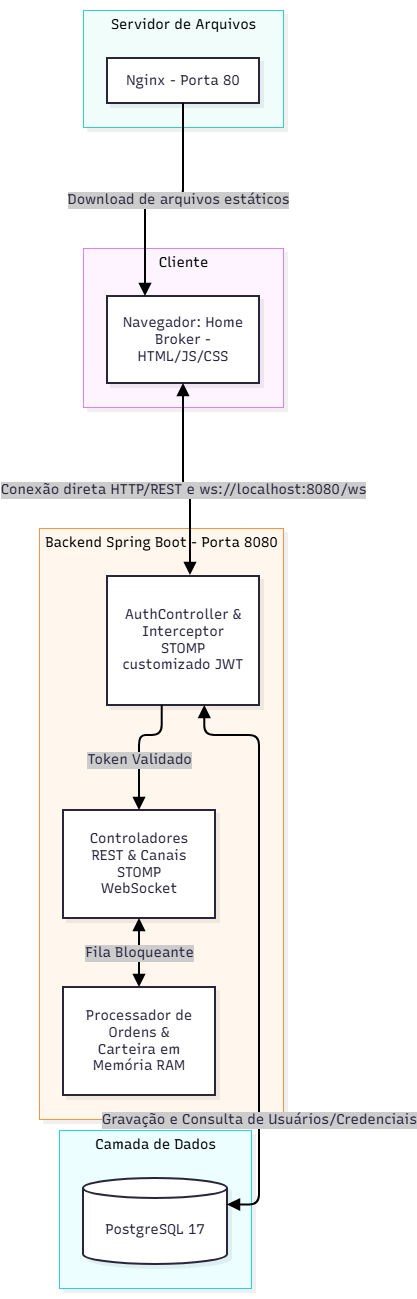
\includegraphics[width=0.35\textwidth]{figs/diagrama de arquitetura.drawio.png}
    \caption{Diagrama de Componentes da Arquitetura do Sistema.}
    \label{fig:arquitetura}
\end{figure}

\subsection{Tecnologias Escolhidas}
A solução foi conteinerizada via Docker, atendendo aos requisitos mínimos. As ferramentas selecionadas são:
\begin{itemize}
    \item \textbf{Backend (Servidor e Matching Engine):} Desenvolvido em Java 21 com Spring Boot 3, utilizando Spring WebSocket/STOMP, Spring Data JPA, Lombok e Maven para gerenciar concorrência e o ciclo de vida das ordens.
    \item \textbf{Frontend (Home Broker):} Desenvolvido em HTML5, CSS3 puro e JavaScript nativo (Vanilla JS), sem frameworks de terceiros, servido de forma estática por um contêiner Nginx na porta 80.
    \item \textbf{Banco de Dados e Cache:} O projeto utiliza PostgreSQL 17 na porta 5432 para persistência. O controle de cache e carteira do protótipo é feito de forma ultrarrápida em memória pelo próprio Java, através de estruturas concorrentes (\texttt{ConcurrentHashMap}), não exigindo o Redis.
\end{itemize}

\subsection{Protocolos de Comunicação}
O sistema utiliza WebSocket nativo em conjunto com o subprotocolo \textbf{STOMP} (em \texttt{ws://localhost:8080/ws}). Os canais implementados incluem:
\begin{itemize}
    \item \textbf{Público (Broadcast):} O canal \texttt{/topic/market} para envio contínuo de eventos do mercado (cotações) a todos os clientes.
    \item \textbf{Privado Ponto-a-Ponto:} Canais como \texttt{/user/queue/orders} (para retornos de aceite/rejeição das ordens) e \texttt{/user/queue/replies} (para listagens de ordens do utilizador).
\end{itemize}
Todas as mensagens transitam através de um envelope padronizado (\texttt{MarketEvent<T>}), contendo metadados cruciais como \texttt{type}, \texttt{requestId}, \texttt{eventId}, \texttt{timestamp} e \texttt{data}. Operações pontuais e estáticas utilizam HTTP/REST tradicional.

\section{Estratégias de Dados, Consistência e Falhas}

\subsection{Banco de Dados e Persistência}
A persistência abrangerá utilizadores, ordens e histórico de negociações no PostgreSQL. O banco relacional foi justificado pela necessidade estrita de transações ACID na gestão dos ativos e capitais dos investidores a longo prazo.

\subsection{Estratégia de Consistência e Concorrência}
O controle de concorrência e consistência do protótipo foi implementado a nível de aplicação em Java, garantindo alta vazão sem corrupção de dados:
\begin{itemize}
    \item \textbf{Idempotência e Ordenação:} O \texttt{OrderService} gera números sequenciais atómicos num bloco sincronizado e utiliza chaves \texttt{userId|clientOrderId} para evitar retransmissões acidentais da mesma ordem.
    \item \textbf{Fila Bloqueante Limitada:} O \texttt{OrderProcessor} gere as ordens através de uma \texttt{LinkedBlockingQueue(10000)} processada em \textit{thread} dedicada. Caso a fila atinja o limite de capacidade, novas ordens recebem a rejeição segura de \texttt{SYSTEM\_BUSY}.
    \item \textbf{Atomicidade de Carteira:} A carteira (\texttt{InMemoryWallet.java}) executa transações de reserva de saldo (para compras) e bloqueio de ações (para vendas) de forma nativamente sincronizada em memória.
\end{itemize}
Para a versão de produção (Parte 2), a persistência total da carteira utilizará travamento pessimista (\textit{Pessimistic Locking} via \texttt{SELECT ... FOR UPDATE}) no banco de dados.

\subsection{Tolerância a Falhas}
Para lidar com quedas de conexão ou reinícios, o sistema prevê:
\begin{itemize}
    \item \textbf{Autenticação \textit{Stateless}:} O acesso e o reconhecimento da sessão utilizam tokens JWT e interceptação nativa de frames STOMP (\texttt{AuthChannelInterceptor.java}), permitindo que o investidor se reconecte sem perder o seu estado de sessão.
    \item \textbf{Prevenção contra Falhas Abruptas:} Em casos de encerramento forçado da aplicação, o sistema registra \textit{logs} avisando sobre as ordens na fila que foram descartadas (\texttt{ORDER\_QUEUE\_DISCARDED}).
\end{itemize}

\subsection{Observabilidade e Testes Automatizados}
Em atendimento ao requisito R13, a implementação foca na qualidade de rastreamento do código:
\begin{itemize}
    \item \textbf{Testes (JUnit 5):} A aplicação já conta com \textit{test suites} consolidados, contemplando simulações de concorrência (\texttt{OrderConcurrencyTest}), limites de fila (\texttt{OrderProcessingTest}), integração STOMP (\texttt{OrderStompIntegrationTest}) e validação atómica da carteira.
    \item \textbf{Observabilidade de Logs:} O fluxo completo de cada ordem registra transições padronizadas nos \textit{logs} (ex: \texttt{ORDER\_RECEIVED} $\rightarrow$ \texttt{ORDER\_ACCEPTED} ou \texttt{ORDER\_REJECTED}), indicando sempre o motivo da falha (como \texttt{INSUFFICIENT\_FUNDS} ou \texttt{INVALID\_FIELDS}).
\end{itemize}



\section{Cronograma de Desenvolvimento}
O cronograma abaixo reflete as atividades distribuídas até as entregas:
\begin{itemize}
    \item \textbf{21/10/2026:} Entrega da Proposta, diagrama arquitetural, infraestrutura em contêineres e Protótipo funcional (login JWT, painel e envio em tempo real via STOMP).
    \item \textbf{Novembro/2026 (Semanas 1-2):} Integração completa do Matching Engine na memória com a base de dados relacional e implementação dos NPCs.
    \item \textbf{Novembro/2026 (Semanas 3-4):} Execução de testes de carga em larga escala, indução de falhas e refatoração arquitetural.
    \item \textbf{30/11/2026:} Apresentação final e entrega do código com documentação.
\end{itemize}

\end{document}